%%%%%%%%%%%%%%%%%%%% author.tex %%%%%%%%%%%%%%%%%%%%%%%%%%%%%%%%%%%
%
% sample root file for your "contribution" to a proceedings volume
%
% Use this file as a template for your own input.
%
%%%%%%%%%%%%%%%% Springer %%%%%%%%%%%%%%%%%%%%%%%%%%%%%%%%%%


\documentclass{svproc}


%%%%%%%% Shorthand definitions %%%%%%%%%%%%%%%%%%%%%%%%%%%%%%%%%%%%%%%%%%%%%%%%%%%%%%%%%%%%%
\newcommand{\kstar}{$k^{*}$\xspace}
\newcommand{\ktrue}{$k^{*}_{\mathrm{True}}$\xspace}
\newcommand{\krec}{$k^{*}_{\mathrm{Rec}}$\xspace}
\newcommand{\minv}{$m_{\mathrm{inv}}$\xspace}
\newcommand{\mt}{$m_{\mathrm{T}}$\xspace}
\newcommand{\pt}{$p_{\mathrm{T}}$\xspace}

\newcommand{\Lam}{$\mathrm{\Lambda}$\xspace}
\newcommand{\ALam}{$\overline{\mathrm{\Lambda}}$\xspace}
\newcommand{\LamALam}{$\mathrm{\Lambda}$ ($\overline{\mathrm{\Lambda}}$)\xspace}

\newcommand{\KchP}{$\mathrm{K^{+}}$\xspace}
\newcommand{\KchM}{$\mathrm{K^{-}}$\xspace}
\newcommand{\Kpm}{$\mathrm{K^{\pm}}$\xspace}

\newcommand{\Ks}{$\mathrm{K^{0}_{S}}$\xspace}

\newcommand{\LamK}{$\mathrm{\Lambda}\mathrm{K}$\xspace}
\newcommand{\ALamAK}{$\overline{\mathrm{\Lambda}}\overline{\mathrm{K}}$\xspace}


\newcommand{\LamKchP}{$\mathrm{\Lambda}\mathrm{K^{+}}$\xspace}
\newcommand{\ALamKchM}{$\overline{\mathrm{\Lambda}}\mathrm{K^{-}}$\xspace}
\newcommand{\LamKchPALamKchM}{$\mathrm{\Lambda}\mathrm{K^{+}}$ ($\overline{\mathrm{\Lambda}}\mathrm{K^{-}}$)\xspace}

\newcommand{\LamKchM}{$\mathrm{\Lambda}\mathrm{K^{-}}$\xspace}
\newcommand{\ALamKchP}{$\overline{\mathrm{\Lambda}}\mathrm{K^{+}}$\xspace}
\newcommand{\LamKchMALamKchP}{$\mathrm{\Lambda}\mathrm{K^{-}}$ ($\overline{\mathrm{\Lambda}}\mathrm{K^{+}}$)\xspace}

\newcommand{\LamKpm}{$\mathrm{\Lambda}\mathrm{K^{\pm}}$\xspace}
\newcommand{\ALamKpm}{$\overline{\mathrm{\Lambda}}\mathrm{K^{\pm}}$\xspace}
\newcommand{\LamALamKpm}{$\mathrm{\Lambda}$($\overline{\mathrm{\Lambda}}$)$\mathrm{K^{\pm}}$\xspace}


\newcommand{\LamKs}{$\mathrm{\Lambda}\mathrm{K^{0}_{S}}$\xspace}
\newcommand{\ALamKs}{$\overline{\mathrm{\Lambda}}\mathrm{K^{0}_{S}}$\xspace}
\newcommand{\LamKsALamKs}{$\mathrm{\Lambda}\mathrm{K^{0}_{S}}$ ($\overline{\mathrm{\Lambda}}\mathrm{K^{0}_{S}}$)\xspace}
\newcommand{\LamALamKs}{$\mathrm{\Lambda}$($\overline{\mathrm{\Lambda}}$)$\mathrm{K^{0}_{S}}$\xspace}

\newcommand{\XiKchP}{$\mathrm{\Xi}^{-}\mathrm{K^{+}}$\xspace}
\newcommand{\AXiKchM}{$\overline{\mathrm{\Xi}}^{+}\mathrm{K^{-}}$\xspace}

\newcommand{\XiKchM}{$\mathrm{\Xi}^{-}\mathrm{K^{-}}$\xspace}
\newcommand{\AXiKchP}{$\overline{\mathrm{\Xi}}^{+}\mathrm{K^{+}}$\xspace}


\newcommand{\XiKpm}{$\mathrm{\Xi}^{-}\mathrm{K^{\pm}}$\xspace}
\newcommand{\AXiKpm}{$\overline{\mathrm{\Xi}}^{+}\mathrm{K^{\pm}}$\xspace}

\newcommand{\Vz}{V$^{0}$\xspace}
%%%%%%%%%%%%%%%%%%%%%%%%%%%%%%%%%%%%%%%%%%%%%%%%%%%%%%%%%%%%%%%%%%%%%%%%%%%%%%%%%%%%%%%%%%%%

\usepackage{xspace}
\usepackage{multirow}
\usepackage{boldline}  % to make lines in table bold
\usepackage{comment}
\usepackage{graphicx,amsmath,amssymb,array,tabularx,url,xspace,subfigure}
\usepackage{relsize} %for \mathlarger
\usepackage{scalerel}  %to use scaleto functionality for math eqns (ex. in exponent of lambda eqn)
\usepackage{subfiles}
\usepackage{arrayjobx} % To use the array structures stored in FitResults_cLamcKch_20180505.tex 
\usepackage{wrapfig}

%
% RECOMMENDED %%%%%%%%%%%%%%%%%%%%%%%%%%%%%%%%%%%%%%%%%%%%%%%%%%%
%

% to typeset URLs, URIs, and DOIs
\usepackage{url}
\def\UrlFont{\rmfamily}

\begin{document}
\mainmatter              % start of a contribution
%
\title{\LamK femtoscopy in Pb--Pb collisions at $\mathbf{\sqrt{{\textit s}_{NN}}} =$ 2.76 TeV measured with ALICE}

%
\titlerunning{\LamK femtoscopy in Pb--Pb collisions}  % abbreviated title (for running head)
%                                     also used for the TOC unless
%                                     \toctitle is used
%
\author{Jesse T. Buxton\inst{1} on behalf of the ALICE Collaboration}
%
\authorrunning{J.~T.~Buxton} % abbreviated author list (for running head)
%
%%%% list of authors for the TOC (use if author list has to be modified)

%
\institute{The Ohio Statue University, Columbus OH 43210, USA,\\
\email{jesse.thomas.buxton@cern.ch}}

\maketitle              % typeset the title of the contribution

\begin{abstract}
The first measurements of the scattering parameters of \LamK pairs in all three charge combinations (\LamKchP, \LamKchM, and \LamKs) are presented.
The results are achieved through a femtoscopic analysis of \LamK correlations in Pb--Pb collisions at $\sqrt{s_{\mathrm{NN}}}$ = 2.76 TeV recorded by ALICE at the LHC.  
The femtoscopic correlations result from strong final-state interactions, and are fit with a parametrization allowing for both the characterization of the pair emission source and the measurement of the scattering parameters for the particle pairs.

\keywords{femtoscopy, heavy-ion collisions}
\end{abstract}
%


%************************************************************************************************************************
%************************************************************************************************************************
\section{Introduction}
\label{sec:Introduction}

Femtoscopy is an experimental method used to study the space--time characteristics of the particle emitting sources in relativistic particle collisions.  
With this method, two- (or many-) particle relative-momentum correlation functions are used to connect the final-state momentum distributions to the space--time distributions of particle emission at freeze-out~\cite{Lisa:2005dd}.
The correlation functions are sensitive to quantum statistics, as well as strong and Coulomb final-state interactions (FSI).  
Thus, femtoscopy can offer a unique environment in which to measure nuclear scattering parameters, many of which are difficult, if not impossible, to measure otherwise.  

%************************************************************************************************************************
%************************************************************************************************************************
\section{Data analysis}
\label{sec:DataAnalysis}

This work reports on the analysis of Pb--Pb collisions at $\sqrt{s_{\mathrm{NN}}}$ = 2.76 TeV produced by the LHC and measured by the ALICE experiment in 2011.
Charged particle tracking was performed using the Time Projection Chamber (TPC) and the Inner Tracking System (ITS).  
Particle identification for reconstructed tracks was carried out using both the TPC and Time-Of-Flight (TOF) detectors in the pseudorapidity range $|\eta| < 0.8$.  
The purities of the \Kpm collections are estimated to be $P_{\mathrm{K}^{\pm}} \approx 97\%$.
Electrically neutral \LamALam and \Ks particles were reconstructed through their weak decays: \Lam $\rightarrow$ p$\pi^{-}$ and \Ks $\rightarrow$ $\pi^{+}\pi^{-}$.
The \Lam and \ALam purities are estimated to be $P_{\mathrm{\Lambda}(\overline{\mathrm{\Lambda}})} \approx 95\%$, and that of the \Ks is $P_{\mathrm{K^{0}_{S}}} \approx 98\%$.
When forming particle pairs, a shared daughter restriction is applied to ensure the first particle in the pair is unique from the second. 
Furthermore, an average separation constraint is imposed to remove splitting and merging effects.


%************************************************************************************************************************
\section{Analysis methods}
\label{sec:AnalysisMethods}
The two-particle correlation function is defined as the ratio of the covariant two-particle and single-particle spectra.
In practice, the correlation function is formed experimentally as $C(k^{*}) = \mathcal{N}\frac{A(k^{*})}{B(k^{*})}$, where $A(k^{*})$ is the signal distribution, $B(k^{*})$ is the reference distribution, and $\mathcal{N}$ is a normalization parameter. 
The signal distribution is the same-event distribution of particle pairs, and the reference distribution is obtained using mixed-event pairs~\cite{Kopylov:1974th}, i.e., particles from a given event are paired with those from another event.

Theoretically, the \LamK correlation function can be described analytically with a model derived by Lednick\'y and Lyuboshitz~\cite{Lednicky:82},
\begin{equation}
\begin{aligned}
C(k^{*})_{\mathrm{Lednick\acute{y}}} = &1 + \sum_{S}\rho_{S}\left[\frac{1}{2}\left|\frac{f^{S}(k^{*})}{R_{\mathrm{inv}}}\right|^2\left(1-\frac{d^{S}_{0}}{2\sqrt{\pi}R_{\mathrm{inv}}}\right) \right. \\
&+ \left. \frac{2\Re f^{S}(k^{*})}{\sqrt{\pi}R_{\mathrm{inv}}}F_{1}(2k^{*}R_{\mathrm{inv}})-\frac{\Im f^{S}(k^{*})}{R_{\mathrm{inv}}}F_{2}(2k^{*}R_{\mathrm{inv}})\right],
\end{aligned}  
\label{eqn:LednickyEqn}
\end{equation}
where $f(k^{*})$ is the complex scattering amplitude, $F_{1}$ and $F_{2}$ are analytic functions, and $R_{\mathrm{inv}}$ is the radius of the spherically symmetric Gaussian distribution assumed for the pair emission source in the pair rest frame.
The complex scattering amplitude is evaluated via the effective range approximation, $f(k^{*}) = \left( \frac{1}{f_{0}} + \frac{1}{2}d_{0}k^{*2} - ik^{*} \right)^{-1}$, where $f_{0}$ is the complex s-wave scattering length and $d_{0}$ is the effective range of the interaction.



%************************************************************************************************************************
\paragraph{Residual correlations}
\label{ResidualCorrelations}

The finally measured correlation function is a combination of the genuine \LamK correlation with contributions from impurities and residual correlations resulting from resonance feed-down~\cite{Kisiel:2014mma},
\begin{equation}
\begin{aligned}
\label{eqn:CfwRes} 
 C_{\mathrm{measured}}(k^{*}_{\Lambda\mathrm{K}}) &= 1 + \lambda'_{\Lambda\mathrm{K}}[C_{\Lambda\mathrm{K}}(k^{*}_{\Lambda\mathrm{K}}) - 1] + \sum\limits_{ij}  \lambda'_{ij}[C_{ij}(k^{*}_{\Lambda\mathrm{K}})-1],
\end{aligned} 
\end{equation}
where $\lambda_{ij}' = \lambda_{\mathrm{Fit}}\lambda_{ij}$, the \LamK term represents the genuine \LamK correlation, and the $ij$ terms denote the contributions from impurities and residual correlations.
The $\lambda_{ij}$ parameters serve as weights dictating the relative strength of each component's contribution to the observed signal, and are estimated using the THERMINATOR 2 and HIJING simulations~\cite{Kisiel:2014mma,Acharya:2018gyz}.
The net contribution from pairs which contain at least one misidentified member are assumed to average to unity.

The main sources of residual correlations in the \LamK systems result from \Lam hyperons which have decayed from $\mathrm{\Sigma}^{0}$, $\mathrm{\Xi}^{0}$, and $\mathrm{\Xi}^{-}$ parents.
When modeling the $\mathrm{\Sigma}^{0}$K and $\mathrm{\Xi}^{0}$K systems, for which the interactions are not known, the source radii and scattering parameters are assume equal to those of the daughter \LamK system.
For modeling the \XiKpm parent contribution, the available experimental \XiKpm data are used.
Each residual component, $C_{ij}(k^{*}_{\Lambda\mathrm{K}})$ in Eq.~\ref{eqn:CfwRes}, is the parent correlation function expressed in terms of the relative momentum of the daughter \LamK pair, and is obtained using a transform matrix generated with the THERMINATOR 2~\cite{Chojnacki:2011hb} simulation (see~\cite{Kisiel:2014mma} for more details).



%************************************************************************************************************************
\paragraph{Non-femtoscopic background}
\label{NonFlatBackground}


A significant non-femtoscopic background is observed in all of the studied \LamK correlations, which is primarily due to particle collimation associated with elliptic flow, and results from mixing events with unlike event planes~\cite{Kisiel:2017}.
These backgrounds are modeled using 6$^{\mathrm{th}}$-order polynomial fits to the THERMINATOR 2 simulation, as shown in Fig.~\ref{fig:BgdswTHERM}, which is then applied as a scale factor in the final fit function.


\begin{figure}[h]
  \centering
  \includegraphics[width=\textwidth]{./Figures/Approved/OtherFormats/EPS/2019-06-11-BgdwFitOnly_RandomEPs_NumWeight1_Full_AllAnwConj_3050.eps}
  \caption[Backgrounds with THERMINATOR 2]
  {
  THERMINATOR 2 simulation (open triangles) with experimental data (closed circles) for the 30--50\% centrality range.  
  Results are shown for \LamKchP (left), \LamKchM (middle), and \LamKs (right).
  A $6^{\mathrm{th}}$-order polynomial fit to the simulation is shown as a dashed curve.  
  This polynomial scaled to match the experimental data is drawn as a solid curve.
  }
  \label{fig:BgdswTHERM}
\end{figure} 

%************************************************************************************************************************
%************************************************************************************************************************
%\clearpage
\section{Results}
\label{sec:Results}

Figure~\ref{fig:LamKFits_3Res} shows experimental \LamK correlation functions with fits for the 0--10\% centrality percentile interval.
All six \LamK systems are fit simultaneously across all centralities, with a single radius and $\lambda_{\mathrm{Fit}}$ parameter for each centrality interval.
Scattering parameters ($\Re f_{0}$, $\Im f_{0}$, $d_{0}$) are shared between pair-conjugate systems, but assumed unique among the different \LamK charge combinations. 
Figure~\ref{fig:ScattParams_3Res} summarizes the extracted \LamK fit parameters.
For all \LamK systems, positive imaginary parts of the scattering lengths, $\Im(f_{0})$, describing the inelastic scattering channels, are extracted. 
More interestingly, the results show that the \LamKchP and \LamKchM systems differ in the sign of the real part, $\Re(f_{0})$, of their scattering lengths, with a negative value for \LamKchP and positive value for \LamKchM (and \LamKs).
The real part of the scattering length describes the effect of the strong interaction, with a positive value signifying an attraction and a negative value signifying a repulsion.
Therefore, the results from this analysis indicate that the strong force is repulsive in the \LamKchP interaction and attractive in the \LamKchM and \LamKs interactions.
\begin{figure}[h!]
  \centering
  \includegraphics[width=\linewidth]{./Figures/Approved/OtherFormats/EPS/2019-06-11-canKStarCfwFits_CombineConj_0010_LabelLines.eps}
  \caption[\LamK data with fits]
  {
  Fit results for the \LamK data in the 0--10\% centrality range; \LamKchP$\oplus$\ALamKchM are shown in the left column, \LamKchM$\oplus$\ALamKchP in the middle, and \LamKs$\oplus$\ALamKs in the right. 
  The curves show the primary \LamK contribution to the fit, i.e., $1 + \lambda'_{\mathrm{\Lambda}\mathrm{K}}C_{\mathrm{\Lambda}\mathrm{K}}$ in Eq.~\ref{eqn:CfwRes} (dotted), the fit to the non-femtoscopic background (dashed), and final fit (solid).
 }
  \label{fig:LamKFits_3Res}
\end{figure}
\begin{figure}[h]
  \centering
  \includegraphics[width=\textwidth]{./Figures/Approved/OtherFormats/EPS/2019-06-11-FinalResults_Comp3An.eps}
  \caption[Extracted Scattering Parameters]
  {
  Extracted fit parameters for all of the \LamK systems.  
  The cross ([A]~=~\cite{Liu:2006xja}) and X (B~=~\cite{Mai:2009ce}) points show theoretical predictions made using chiral perturbation theory.
  }
  \label{fig:ScattParams_3Res}
\end{figure}





%************************************************************************************************************************
%************************************************************************************************************************
\section{Summary}
\label{sec:Summary}
Results from a femtoscopic analysis of \LamK correlations in Pb--Pb collisions at $\sqrt{s_{\mathrm{NN}}}$ = 2.76 TeV measured by the ALICE experiment at the LHC have been presented.
The femtoscopic radii, $\lambda$ parameters, and scattering parameters were extracted from one-dimensional correlation functions in terms of the invariant momentum difference.
Striking differences are observed in the \LamKchP, \LamKchM, and \LamKs correlation functions, and the extracted scattering parameters indicate that the strong force is repulsive in the \LamKchP interaction and attractive in the \LamKchM and \LamKs interactions.
This effect could be due to different quark--antiquark interactions between the pairs, or from different net strangeness for each system. 

%%%%%%%% Bibliography (In case of using bibtex generate the bbl requested by arXiv)
\bibliographystyle{spphys.bst}   % Remember we use title in the biblio
\bibliography{LamK_bibfile}
%\input {bibliography.tex}  

%%%%%%%%% appendix with author list
\newpage
\appendix
%
%% Following lines needed so, for instance, Fig D.1(a) not printed as simply 1(a) when referenced
\renewcommand{\thesubfigure}{\thefigure(\alph{subfigure})}
\makeatletter
\renewcommand{\p@subfigure}{}
\renewcommand{\@thesubfigure}{(\alph{subfigure})\hskip\subfiglabelskip}
%\input{}               %%%%%%%%%%% put your appendices here
%


%************************************************************************************************************************



\end{document}
